\section{General Practices}
\label{imp:general_practices}

Software development is hard and, at times, frustrating. The following
general practices should allow for greater productivity, higher
quality software and less frustration involved in the process of creating it.

\subsection{Documenting Functions}
When writing code, it is valuable to spend time making sure the
code is readable. One way of increasing readability is to provide comments
to non-trivial code samples. Doing this, the programmer will not only
help himself, but also his peers, in later reading and understanding of the code.

When providing comments to top-level functions in C\#, it is
recommended to do so by using XML comments as seen in
\cref{fig:xml_comments_example}. By structuring the comments above a
corresponding top-level function, other software can present nicely
viewable code documentation.

\begin{lstlisting}[caption = {Example of XML-comments on top of C\# function.}, label={fig:xml_comments_example}]
/// <summary>
/// Gets list of unique tracks from JSON
/// </summary>
/// <param name="jsonCode">JSON collection of tracks</param>
/// <returns>List of tracks contained in JSON</returns>
private List<Track> GetTracks(JToken jsonCode) {
\end{lstlisting}


\chapter{Design Patterns}

\section{Model View Viewmodel}

This project is both on the client and on the server structured using
the Model View ViewModel (MVVM) pattern. The core idea in MVVM is to
separate the presentation layer, the view in MVVM, from the model
layer, the model in MVVM. This separation is done by introducing a
ViewModel layer. The ViewModel exposes data from the model to the view
in such a way that the view layer never has any knowledge about the
model layer.

This pattern is used mainly because the frameworks used on the client
and server are designed to be structured using this pattern. Other
similar patterns such as Model View Controller (MVC) could
theoretically also have been used, but doing so would go against some
of the principles the frameworks used are based upon.

\section{Singleton Pattern}

The singleton pattern is used whenever there should only ever be one
instance of a class. The pattern is often implemented as a static
method on the class, that instantiates the class on the first call,
and on later calls returns the created instance of the class.

This pattern is used in SpotifyDotNet, the libspotify wrapper, used in
this project. Because it is only possible to be logged in one user at
a time, the SpotifyLoggedIn class implements the singleton pattern.

\section{Dependency Injection}

Dependency Injection is a design pattern that helps to reduce coupling
between different components in a software program. The main idea is
to have components not depend on concrete dependencies but instead
depend on abstractions of dependencies. Doing this, dependencies can
be dynamically changed during runtime as long as their abstractions
match up.

In this project the StructureMap framework is used to reduce
boilerplate and ease the implementation of Dependency Injection.


\chapter{Client}

This chapter describes the client side of the solution, and which frameworks are used in this project, in order to design a cross platform mobile application. 

\section{Native Application Development Framework}
\label{par:native_application_development_framework}

Many native application development frameworks exist, including Android SDK, iOS SDK, Windows Phone SDK, Qt, Xamarin.Forms and more. They each have their different characteristics. Android SDK makes it possible to build Android applications. The applications are written in the programming language Java. Similarly you can use iOS SDK to build iOS applications and Windows Phone SDK to build Windows Phone applications using Objective C or Swift, and C\# respectively. Qt is cross platform, so the application written using Qt can run on a variety of systems including Android, iOS and Windows Phone. Qt is written in the programming language C++. Xamarin.Forms is also cross platform and is written in C\#.

With so many good frameworks it is hard to choose one to go with. Fortunately the semester description helps to decide by specifying that all programming should be in C\#. This narrows the possibilities of frameworks down to Xamarin.Forms or limiting the platforms to only Windows Phone devices.

Limiting the application to only Windows Phone devices would drastically limit the amount of devices which could run the application.

Xamarin.Forms makes it possible to write an application in C\# and run it on iOS, Android and Windows Phone. The application will look differently on the three platforms, but they will feel native on each of the platforms.

Because Xamarin.Forms enables native applications for all three large mobile platforms, the client application can reach a large user base. The client application is therefore chosen to be written using the Xamarin.Forms framework.
%%% Local Variables:
%%% mode: latex
%%% TeX-master: "../../master"
%%% End:


\chapter{Server}

This chapter describes how the server side functionality of the solution is implemented. It is described how the third party frameworks are used to obtain meta data, and stream the music. Additionally, the steps which were taken to ensure the quality of the solution will be characterised.

\section{White- and Black-list}

An obvoius implementation of these concepts is to white- and black-list specific tracks, this is a solution but to ease the process of making such extensive restriction, for the administrator, a possiblity of making more coarse restrictions would be beneficial. These restrictions is based on metadata related to the tracks, the artist of the track, the genre of the track or some signature tags. Spotify provides the artist and occasionaly the genre, the tags should be provided by another third party database of tags, like MusicBrainz. To ensure that the same track is found across both databases, an ISRC \footnote{International Standard Recording Code\cite{isrc}} is provided from Spotify database.

This is implemented as a list of predicates, that each individual track must meet in order to be added to the playlist. These predicates ad to evaluate the artists of the track, if a black listed artist occurs on the track, lets say "Justin Bieber", the track is discarded, before being added, although when the user searching for a track, in convience of the user, the track can be marked as "filteredout" to explicitly state that the track where found but is not allowed to played at the specific venue, hopefully minimizing any confusions made during the search phase.


\section{Duplicates in the music catalog - Similar tracks variable lenght}
\label{sub:duplicates}

Some tracks in the music catalogue might be "duplicates", while maybe variyng in lenght, the track might the lyrics and the music is quite similar or simply identical. One imediate partwise solution is to compare the IRSC of the track, if they match one could discard either one of them, shortest duration might by most desirable, in the context of a venue with many music request.

more optimisations is needed though.
\section{Access to Spotify}
\label{sub:Access_to_Spotify}

As it is now established that Spotify is the music catalogue of choice, it is important to think of ways to access their data. As of this report, two main APIs are available: Spotify Web API and libspotify. They each have their benefits and limitations.

\subsection{Spotify Web API}
\label{techPlat:music_catalog_web_api}

The Web API is the easiest of the two to work with. It is not needed to login with a Spotify account to use this API, however when the user is authorized, rate limits improve. The API is accessed as a simple REST based interface to nearly all their data. That is, tracks, albums, artists, playlists, user profiles, album art and track previews are all accessible. Notice that this is only metadata about tracks, albums etc. Besides the track previews, no music can be streamed using this API.

So the price of simplicity and ease of use is the limitation of only being allowed to access metadata.

\subsection{Libspotify}
\label{techPlat:music_catalog_libspotify}

Libspotify is a C library written and distributed by Spotify. It is more feature-rich and complex than the Web API. The library can access any data that the official Spotify client can. In fact, the official Spotify client uses libspotify. This implies that both accessing metadata, searching and music streaming is possible. The downside to this more powerful library is the requirement of a Spotify Premium account and the complexity of managing memory and threads.

\subsection{Conclusion}
\label{ssub:music_catalog_conclusion}

Based on the knowledge acquired above it is determined that the web API is best used for retrieving metadata by searching Spotify's data. It is easily integrated in different contexts, as the only requirement is an internet connection.

Libspotify is best used in a context where playback of tracks are needed and the requirement of a Spotify Premium account is no problem.
%%% Local Variables:
%%% mode: latex
%%% TeX-master: "../../master"
%%% End:


\section{Spotify Web API}
\label{imp:spotify_web_api}
This section provides information on the structure of the classes are build around Spotify Web API \sinote{and possibly the whole project}. It will describe the considerations and approaches that has been taken, when designing the architecture.

When using the Web API to search on Spotify, three different items can be found: Track, Album and Artist. These three items are all identified by a unique ID from Spotify, which is what is also used as the id for the item in this project. A small problem occurs in the implementation of this search since it is required to specify what kind of item is being searched for. The user, although always eventually looking for a track, does not always find the track directly via the title, but often via the artist by whom it was created or album on which the track is placed. It was therefore chosen that each search requires a specification on what type item that is being searched for. To minimize the requirements for the user, it was decided that the user, should not specify what item they are searching, but rather they should write the search string, and get a complete list of the results for all items represented. Therefore it has been implemented, that it is possible, when creating a Search object, to specify from an enum which of the three items or all three are being searched for. When choosing all three, which is what is done for the users searches, three individual searches are created and the results are represented in a complete structure shown in \cref{fig:WebAPIUML}.

\begin{figure}[H]
\centering
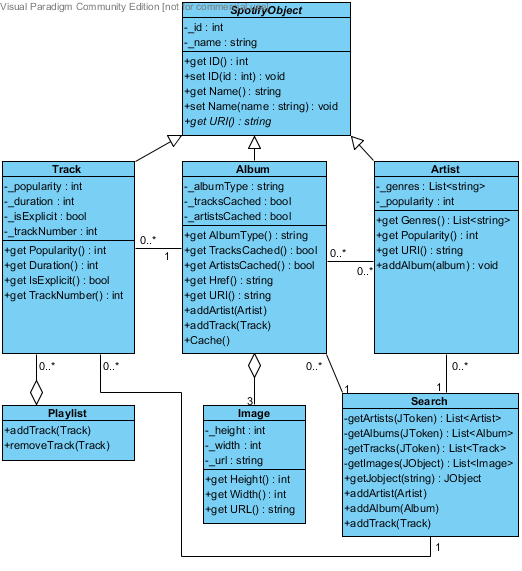
\includegraphics[width=\textwidth]{Images/WebAPIUML.png}
\caption{A class diagram showing the class structure of the results generated from a search}
\label{fig:WebAPIUML}
\end{figure}

\subsection{Lazy Searching}
\sinote{hvordan gør vi dette? det står lidt løst}

To minimize the amount of data being downloaded when using the web API, a strategy was developed for only requesting data from Spotify when it is actually needed. Initially, \sinote{Jeg skal lige have snakket med Jens for at skrive mere}

It was decided to have a minimal data download approach when designing the web API. This was done on the bases of the assumption that this API would most likely be the system used for searching for new tracks on the mobile front-end application. Since mobile phones still have limited data access, it is preferable for the user to use as little data as possible. This approach results in only three searches being done, one for each item type. Other requests are not done until other information about the item is needed. Furthermore this approach also results in all information being stored in the objects locally. It will be saved until the search object is removed, and the user hopefully has found his or her track.

One search usually searches for all three different item types, track, album and artist, and present these to the user. Not all information about the artists and albums can be gathered from the json code received from these three initial searches. Albums does not have information about it tracks nor its artists initially, and an artist does not have information about its albums. The minimal data approach was therefore combined with another idea, data just in time. This was done since the user normally only wants information from one type of item, and not the two remaining types. It would therefore be undesirable for the user to wait, for all information for every item to be downloaded. This also fits very well with the minimal data approach since this minimize the amount of data requested, if the user does not look though all items in the search. The information not received from the initial searches, is therefore only requested from Spotify when the get method for the properties on items are called. To keep faithful to the minimal data approach this information is cached to the application and saved in the object structure so that the data does not have to be downloaded again.


\section{Libspotify Abstraction}
As stated in \cref{music_catalog_libspotify} the only way to stream tracks off Spotify is using the C library libspotify. Being written as a C library, one has to take care of managing memory allocation correctly in order to avoid runtime exceptions while using libspotify.

To make it harder to cause these runtime errors and to ease interoperability in the C\# environment, a C\# library can be written that abstracts the error prone elements of C programs away. The C\# library \enquote{SpotifyDotNet} developed for use in the software described in this paper, does just that.

\subsection{Abstracting Low-level C Concepts Away}
\label{libspotify:abstracting_low_level_c_concepts_away}

The goal of the SpofityDotNet library is to minimize runtime exceptions caused by memory related errors. To do this, the error prone unmanaged C code has to be accessed as secure managed C\# code.

SpotifyDotNet uses existing bindings, hosted on \url{http://libspotifydotnet.codeplex.com/}, to interface with libspotify from C\#. As an example let's look at the login function from libspotify. See \cref{fig:loginC}. The corresponding binding can be seen in \cref{fig:loginCsharp}. As can be seen, a C pointer maps directly to an IntPtr struct in C\#. \lstinline|const char*| becomes a common string object in C\#. A C bool is simply a C\# bool.

\begin{lstlisting}[caption = {Libspotify login function prototype - C}, label = {fig:loginC}]
sp_error sp_session_login ( sp_session *session,
                            const char *username,
                            const char *password,
                            bool remember_me,
                            const char *blob
                          )
\end{lstlisting}

\begin{lstlisting}[caption = {Login method using a external implementation from libspotify.dll - C\#}, label={fig:loginCsharp}]
public static extern sp_error sp_session_login ( IntPtr sessionPtr,
                                                 string username,
                                                 string password,
                                                 bool rememberMe,
                                                 string blob
                                               )
\end{lstlisting}

However this is not abstracted enough. To the user of the library, no pointers should be visible. This is solved by encapsulating state and data inside the Spotify class. This class is the entry point to using libspotify in C\#. See \cref{fig:spotifydotnet_class} for complete class diagrams. The main operation on the class is the Login method. This method is asynchronous so it will utilise the C\# feature of Tasks. A Task is simply a promise that something will happen in the future. In this context, the login method returns an \lstinline|Task<Tuple<SpotifyLoggedIn,LoginState>>|. So the login method promises that it will return \lstinline|Tuple<SpotifyLoggedIn,LoginState>| at some time in the future. When login has occurred, LoginState will describe the state of the login process. If LoginState is \enquote{OK}, the login was successful and SpotifyLoggedIn will be non-null. If LoginState was anything other than \enquote{OK}, SpotifyLoggedin would be null. The SpotifyLoggedIn object sent with the login method, exposes all methods that are available when logged into Spotify. See \cref{fig:spotifydotnet_class}. By only exposing the SpotifyLoggedIn object when correctly logged in, certain errors like searching without being logged in, can be detected at compile time.

\begin{figure}
  \centering
  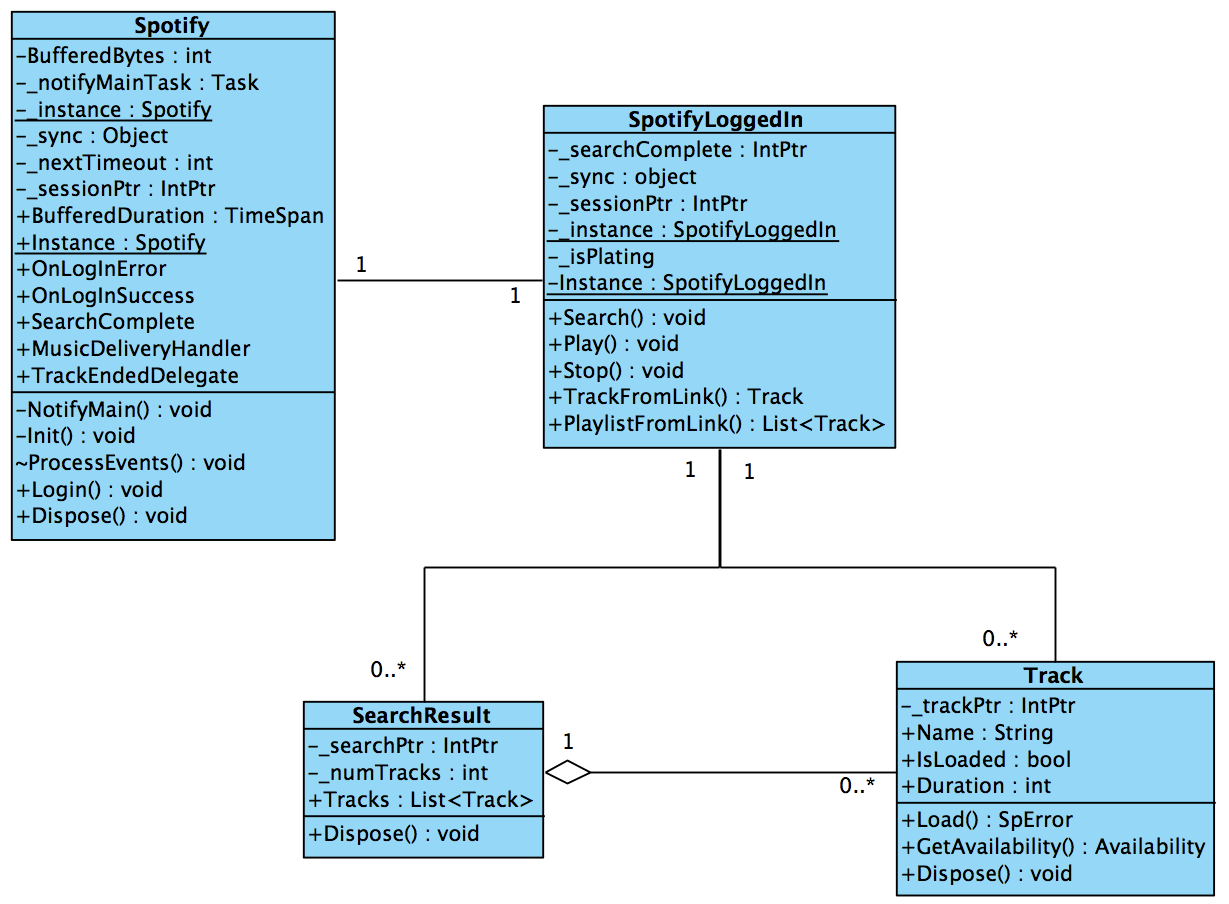
\includegraphics[width=1.2\linewidth]{spotifydotnetClass.png}
  \caption{Class diagram of SpotifyDotNet library}
  \label{fig:spotifydotnet_class}
\end{figure}

\subsection{Making it Thread-safe}
\label{libspotify:making_it_thread_safe}

As stated in~\cite{spotifyLibspotifyFAQ}, libspotify is not thread safe. This is solved in SpotifyDotNet by using locks around non thread safe code. This is easily done in C\# using the \enquote{lock} keyword as seen in \cref{lst:lock_keyword}. Locks are a way to avoid race conditions i.e. threads modifying the same chunk of memory at the same time. Race conditions lead to non-deterministic results, which is always to be avoided. Locks solve this issue by synchronizing the threads. Whatever code blocks are wrapped around locks can only be accessed by one thread at a time.

\begin{lstlisting}[caption = {Example of using the lock keyword in C\#. \enquote{\_sync} is an object used to store the lock state}, label = {lst:lock_keyword}]
lock(_sync) {
  thisWillRunThreadSafe();
}
\end{lstlisting}

To the user of SpotifyDotNet, no errors related to threads can occur when using the library on multiple threads.


\section{Backend Server}
\label{imp:backendServer}

As described in \cref{techPlat:backendServer}, HTTP endpoints must be
available to the client from the server. This section presents all the
available endpoints and describes key implementation
details. Additionally the details of the playback of tracks from
Spotify are detailed.

Nancy, a lightweight framework for building HTTP services in C\# is leveraged
to cut down development time.

\subsection{Checking-in}
For checking in to a venue, the client has to send a unique user ID to
the endpoint shown in \cref{lst:endpoint_checkin}

\begin{lstlisting}[label={lst:endpoint_checkin}, caption={HTTP endpoint allowing client to check-in to a venue. Text surrounded by curly brackets are parameters.}]
http://server:port/checkin/{userID}
\end{lstlisting}

\subsubsection{Returns}
"OK" when action is completed.

\subsection{Searching}
To search, just a search query is needed.

\begin{lstlisting}[label={lst:endpoint_search}, caption={Text surrounded by curly brackets are parameters.}]
http://server:port/search/{query}
\end{lstlisting}

\begin{lstlisting}[label={lst:endpoint_search_offset}, caption={Text surrounded by curly brackets are parameters.}]
http://server:port/search/{query}/{offset}
\end{lstlisting}

\subsubsection{Returns}
Tracks on Spotify that matches the query requested, with a possible offset for more results. This is formatted in JSON.

\subsection{Playlist}

\begin{lstlisting}[label={lst:endpoint_playlist}, caption={Text surrounded by curly brackets are parameters.}]
http://server:port/playlist
\end{lstlisting}

\subsubsection{Returns}
The current and sorted playlist is returned to the client in JSON.

\subsection{Now playing}

\begin{lstlisting}[label={lst:endpoint_nowplaying}, caption={Text surrounded by curly brackets are parameters.}]
http://server:port/nowplaying
\end{lstlisting}

\subsubsection{Returns}
The current playing track or "Nothing currently playing" is returned to the client in JSON.

\subsection{Voting}

\begin{lstlisting}[label={lst:endpoint_vote}, caption={Text surrounded by curly brackets are parameters.}]
http://server:port/vote/{userID}/{trackId}
\end{lstlisting}

\subsection{Volume}

\begin{lstlisting}[label={lst:endpoint_volume}, caption={Text surrounded by curly brackets are parameters.}]
http://server:port/volume/{volPercent}/{userId}
\end{lstlisting}

\subsubsection{Returns}
The average percentage of volume of all users is returned to the client.

\subsection{Check-out}

\begin{lstlisting}[label={lst:endpoint_checkout}, caption={Text surrounded by curly brackets are parameters.}]
http://server:port/checkout/{userID}
\end{lstlisting}

\subsubsection{Returns}
"Success" or "Failure" depending on is the action was successful.

\subsubsection{Returns}
"OK" when action is completed.

%%% Local Variables:
%%% mode: latex
%%% TeX-master: "../../master"
%%% End:


\chapter{Quality Assurance}
This chapter presents methods to evaluate the quality of a software system. These methods aid in performing usability tests and extracting the necessary conclusions out of these.

\input{Chapters/Implementation/QualityAssurance/testMethods.tex}
%\input{Chapters/QualityAssurance/complexityOfAlgorithms.tex}
\section{Usability}
\label{sub:usability}

Usability can be defined as \enquote{when a product or service is truly usable, the user can do what he or she wants to do, the way he or she expects to be able to do it, without hindrance, hesitation, or questions}~\cite{RubinChisnellSpool08}.

There are different ways of evaluating the usability of a product. The two, being looked at in this report, are \textit{empirical} and \textit{heuristic} testing. The goal of a usability test is to come up with a list of usability problems. A usability problem is a deficiency in a product that makes it less usable. An example of a usability problem is when a simple task like deleting an email takes an inappropriate amount of effort.

\subsection{Usability Testing}
\label{sub:usabilityTesting}
Usability testing is an empirical technique used to evaluate a product by testing it with users in focus. An example of an empirical technique could be testing the interface, by making the users execute some tasks while commenting on the interface. When there are referred to usability testing it is this technique that are meant, and not the general principle of testing the user interface. The purpose of the test is to determine usability problems with the product~\cite{RubinChisnellSpool08}. In this report the term \emph{usability testing} is used to refer to the process of testing with users, and not as a general term for testing usability. The test is intended to be realistic and simulate potential scenarios that can happen while using the product. A usability test is usually performed with a representative user performing a series of tasks. A test monitor will watch the participant completing the tasks without interrupting the participant in doing the tasks. While the participant is solving the task, a data logger is noting how the participant is solving the tasks given and the problems faced doing so.

After a usability test is conducted, the results must be analysed and documented. In most usability testing analysis methods, this involves spending a lot of time doing video data analysis. In this project, a newer method called \enquote{Instant Data Analysis} (IDA)~\cite{kjeldskov2004instant} was used. This method seeks to reduce the resources required to conduct the analysis. In IDA the procedure is as follows. After the test, a one hour brainstorm session between the data logger and test monitor has to occur. A facilitator manages the brainstorm and writes usability problems on a whiteboard. After the brainstorm, the facilitator spends 1-1.5 hours writing usability problems into a ranked list. Using IDA reduces the time spent on analyzing to 10\% compared to the traditional video analysis method~\cite{kjeldskov2004instant}. While still finding 85\% of the critical problems.

\subsection{Heuristic Evaluation}
Heuristic evaluation is a method to inspect usability of computer
software. It involves a number of evaluators that are presented with
an interface design and asked to comment on it. This is used to come
up with a list of usability problems in a user interface design. This
information can be used as part of an iterative design process to make the design more usable.

Heuristic evaluation is usually done by judging how the software meets
certain predetermined heuristics. A set of ten heuristics
is presented in \citetitle{Nielsen1994}. These are as follows

\begin{enumerate}
  \item Visibility of system status
  \item Match between system and the real world
  \item User control and freedom
  \item Consistency and standards
  \item Error prevention
  \item Recognition rather than recall
  \item Flexibility and efficiency of use
  \item Aesthetic and minimalist design
  \item Help users recognise, diagnose, and recover from errors
  \item Help and documentation
\end{enumerate}

The method is not good for finding all problems; an individual person
can only find between 20\% and 51\% of all
problems~\cite{Nielsen1990}. Therefore it is recommended that multiple
people conduct the evaluation independently of one another. The
results can then be merged together.It is recommended in \citetitle{Nielsen1990} that 3 to 5 people do independent evaluation to get good coverage.

A disadvantage of heuristic evaluation is that it sometimes identifies usability problems without providing direct suggestions for how to solve them~\cite{Nielsen1990}. The method is biased by the current mindset of the evaluators and normally does not generate breakthroughs in the evaluated design. This technique has been researched and described, to compare against other general usability testing methods. 



\section{Usability Test in Laboratory}
Usability testing in this project will be used as a tool to test and
ensure quality of the user interface of the client application. An empirical evaluation was chosen over heuristic evaluation since it would get more data on usability problems. It would also evaluate the program with potential users, this would give assurance that the program lives up to the users' expectation and requirements. The tests will be performed on
typical users that were determined in \cref{userInterviews}, who are
representative end users of the product. It was chosen to conduct the
test in a laboratory since it is easy to create a controllable
environment and record video. Because of the limited time, it was
chosen to do IDA as described in \cref{sub:usabilityTesting}.  This will not find as many usability problems as video analysis, but it will only take 10\% of the time~\cite{kjeldskov2004instant}.

\subsection{Procedure}
\begin{figure}[hbtp]
  \centering
  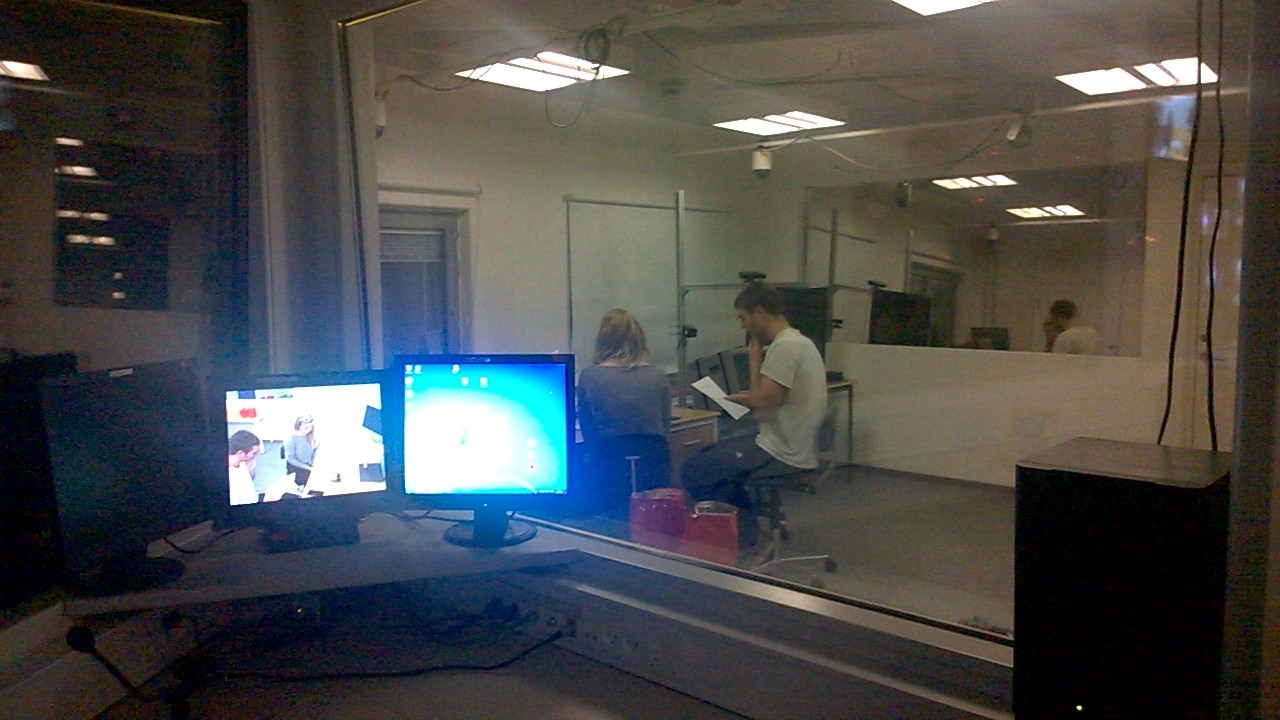
\includegraphics[width=1\linewidth]{subjectRoom}
  \caption{View from the control room into the subject room.}\label{fig:subjectRoom}
\end{figure}

The tests were conducted at the usability laboratory in the Department of Computer Science at Aalborg University. On \cref{fig:subjectRoom} is a picture of the usability laboratory. The laboratory is split into three different rooms: control room, subject room and observer room. The test was done on a smartphone of the model OnePlus One. This was the phone that was available at hand and it is equipped with a powerful processor. The members of the group were assigned different roles; two persons were assigned as alternating datalogger in the observer room and leader in the subject room. Another person was datalogger at all tests also in the observer room taking notes. A fourth person was responsible for entertaining the test subjects when they were not being tested and also driving the subjects that needed help arriving at the testing location. The fifth person was the video operator and was responsible for recording and mixing the video feeds from the subject room. The last person was assigned the role of social environment simulator. He was responsible for simulating other users actively using the test application, by adding multiple tracks to the playlist. This was done in order to make the usage of the application more realistic. The application tries to make a social experience and ideally there would be more than one person interacting with the server at a time. This tasks was though a fairly trivial task since all tracks and when to add them where decided before the tests. This last person therefore also acted as a datalogger most of the time.

The tests was done as think-aloud sessions. At the start of a test, an introduction was read out loud to the test
subject. The introduction can be found in
\cref{usabilityTestIntro}. The subject would then answer a
questionnaire which can be found in \cref{tab:participants}. The test
proceeded with the test subjects reading a premade task and then
trying to accomplish that task. All tasks can be seen in \cref{usability_tasks}. The task description has to be detailed enough, so that no excessive information about the test program is exposed~\cite{RubinChisnellSpool08}. The tasks was designed to take about 15 min. After the tasks was completed there was extra time for a free-form discussion about the application. In the end each test ended up in the range of 15 to 30 minutes. This difference in time came mainly from the free-form discussion.

\subsection{Participants}
It was decided to test with users, because it would give an indication
of how real end-users use the system. Since the system is to be used
in a bar and is targeted for students, students were chosen as test
subjects. The subjects were recruited from the user interviews
described in \cref{userInterviews}. \Cref{tab:participants} presents
information gathered from the before mentioned questionnaire.

\begin{table}[hbtp]
    \centering
    \tabcolsep=0.10cm
    \begin{tabular}{lccccr}
        \toprule
        \textbf{\#} & \textbf{Sex} & \textbf{Age} & \textbf{Field of study} &
        \textbf{Smartphone experience} & \textbf{Primary phone} \\
        \midrule
        1                   & F               & 20           & Techno-Anthropology       & Experienced                    & iOS                    \\
        2                   & F               & 19           & Mathematics             & Intermediate                   & Android, iOS           \\
        3                   & F               & 20           & SIV Spanish             & Experienced                    & iOS                    \\
        4                   & F               & 22           & Electronics and IT      & Intermediate                   & Android                \\
        5                   & M               & 20           & Electronics and
        IT      & Experienced                    & Android                \\
        \bottomrule
    \end{tabular}
    \caption{Participants.}\label{tab:participants}
\end{table}

\subsection{Data Collection}
The screen of the phone was recorded with software on the phone. The
video feeds from the two cameras in the test room were recorded to a
DVD. The data logger was taking notes while the test subjects were
performing their tasks.

\subsection{Data Analysis}
It was not possible to conduct the IDA brainstorming and data analysis
sessions the same day as the tests, since the subjects were only able
to conduct testing after normal working hours, and it would be too
late in the evening after the tests, to ensure a good quality of the
sessions. This presented a problem, since IDA normally requires these
sessions, to be done on the same day as the test. Since it was not
possible to move the tests, it was decided to compensate for this with
multiple dataloggers. Normally IDA only requires one person to be
assigned as a datalogger. In the tests conducted two people would at
any time be dedicated dataloggers. The environment simulator would
furthermore, most of the time, also act as a datalogger, resulting in
2-3 dataloggers during the tests. It was assessed that this would be
enough, to compensate for the brainstorm and data analysis sessions
delay. The session was conducted as the first thing the next morning.

The data analysis can be split into four different areas; brainstorm, task review, note review and severity rating. These four areas where created according to the the analysis part of IDA~\cite{Kjeldskov2004}.

\subsubsection{Brainstorm}
First, the brainstorm session was conducted. During the brainstorm
session, one person was assigned the role of IDA facilitator. After this, everyone in the group stated all problems found during the tests they could find from memory.

\subsubsection{Task Review}
After the brainstorm, the task review session was conducted. Here, the
tasks were taken in use for remembering additional problems for
specific tasks. The IDA facilitator was responsible for reading the
questions aloud and writing down every problem which was found.

\subsubsection{Note Review}
In the note review session, the notes taken by the dataloggers were
taken in use. Here, the IDA facilitator and the dataloggers converted
the notes taken by the dataloggers into specific problems. This was
done in collaboration with the rest of the group, since these notes
could, and did, emphasise additional problems. All problems were written down.

\subsubsection{Severity Rating}
During this session, every problem found in the earlier sessions was
discussed. Problems that could, were organised into one general problem and all these general problems were put on a list.

After this, the data was organised into a list of problems. The
problems were sorted into three categories from
\citetitle{molich2007usable}: Minor, serious or critical.
A minor problem is when the user hesitates or is delayed for a few
minutes. A serious problem is when the user is delayed for more time
or expresses irritation. A critical problem is when the user comes to a full stop and cannot continue without human intervention.

In total, the analysis lasted about 1½ hours. During the sessions,
screen recordings and the DVD was used during the analysis, when there
was confusion about what happened at the test. The result of the
analysis was a list of problems. On this list, the ranking of the problem, a problem description and which test persons suffered from the problem is noted.

\subsubsection{Serious}
\textbf{Problem \#1 - Vote confusion. The user does not know how votes work, what the person has voted for and when the person has voted. Test persons \#1, \#2, \#3, \#4 and \#5.}\\
All test persons were unsure how votes work. They did not receive any indication about how many votes they had. All of them were also not sure which track they had currently voted on. Also, no confirmation upon voting was displayed.\\

\noindent\textbf{Problem \#2 - Confusion about multiple copies of the same song on the playlist and now playing. Test persons \#2, \#4 and \#5.}\\
When in the playlist view, a track would both be contained in the playlist of the venue while at the same time being displayed as now playing. An example of this can be seen in \cref{fig:twoSongs}. This would confuse the test persons, and they would get unsure about which end of the playlist was ranked highest.\\

\begin{figure}[hbtp]
  \centering
  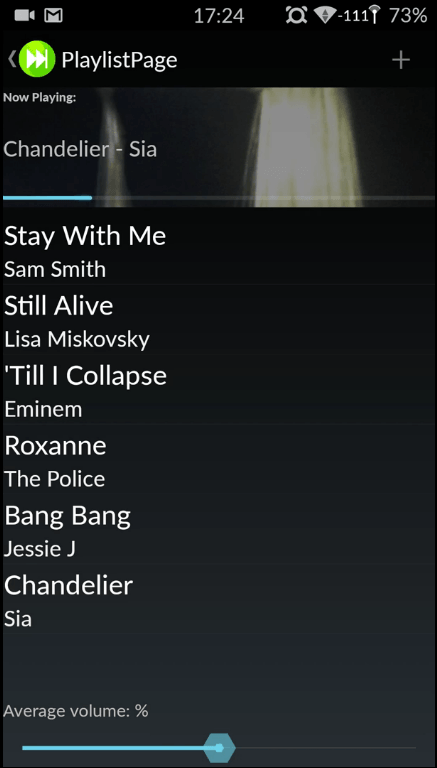
\includegraphics[width=0.3\linewidth]{twoSongs}
  \caption{Chandelier by Sia is displayed as currently playing, but is still at the bottom of the playlist.}\label{fig:twoSongs}
\end{figure}

\noindent\textbf{Problem \#3 - The user is confused on how well tracks are doing on the playlist. Test persons \#1, \#2 and \#5.}\\
This problem relates to problem \#2. There was no indication about how the tracks in the playlist are ordered. When asked about which track would be played next, some test persons had difficulties determining this.\\

\subsubsection{Minor}
\textbf{Problem \#4 - Missing confirmation when adding tracks on search. Test persons \#1, \#3, \#4 and \#5.}\\
When pressing on a track after searching for it, no feedback was given whether the track was successfully voted for. It was just marked blue as seen on \cref{fig:search}\\

\begin{figure}[hbtp]
  \centering
  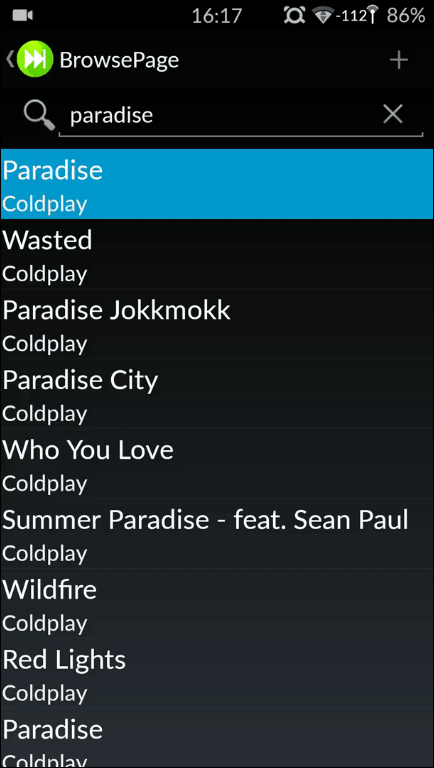
\includegraphics[width=0.3\linewidth]{search}
  \caption{When tapping a track on the search view to vote, the track
    would be marked blue, but no further indication of a successful
    vote would appear.}\label{fig:search}
\end{figure}

\noindent\textbf{Problem \#5 - Check-in confusion, does not know whether the person is checked
    in or not. Test persons \#1, \#2 and \#3.}\\
  When pressing on a venue to check in, test subjects would wait for
  something to happen in the app, even though the app was already
  checked in. There was no confirmation upon a successful check in.\\

\noindent\textbf{Problem \#6 - Did not know in which direction to swipe on the start page. Test
    persons \#2, \#4 and \#5.}\\
  When presented with the start page, a arrow and a corresponding text
  would indicate in which direction the test subject would have to
  swipe in order to get to the check in page. As seen in fig \cref{fig:swipe} this arrow was confusingly
  directed, which caused some test subjects to swipe in the wrong direction.\\

\begin{figure}[hbtp]
  \centering
  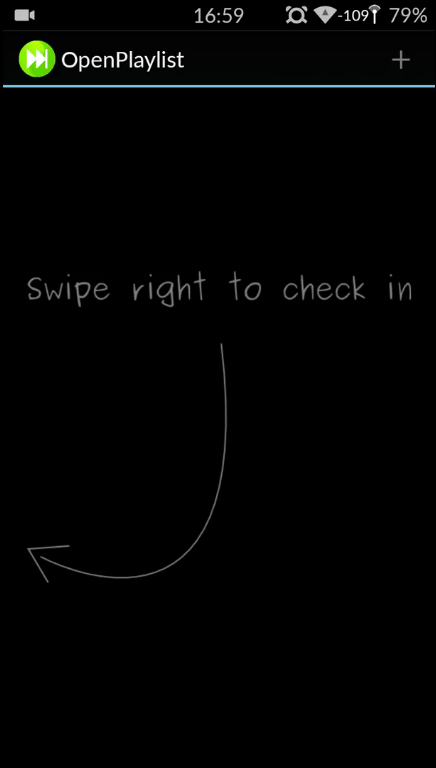
\includegraphics[width=0.3\linewidth]{swipe}
  \caption{Confusing arrow, which made some of the subject swipe in the wrong direction.}\label{fig:swipe}
\end{figure}

\noindent\textbf{Problem \#7 - Search confusion, does not know whether and when a search is
    happening. Test persons \#1 and \#5.}\\
  When pressing the search button, some feedback was given that the
  application was performing the search, but this was not standing out
  to the user. The user would therefore click twice on the search button.\\

\noindent\textbf{Problem \#8 - Loading indicator confuses user. They thought it was their actions
    that influenced the loading indicator. Test person \#2.}\\
  In the application, a automatic refresh of the playlist and
  now playing would update every 3 seconds. Whenever this automatic
  refresh happened, a small loading indicator would rotate. This
  indicator would show even if the user had not actively affected the application.\\

\noindent\textbf{Problem \#9 - Expected \enquote{clear search button}
  to remove results and bring user back to the playlist. Test person \#2.}\\
  When the test subject clicked on the clear button of the search bar,
  the subject was confused that just the text in the search bar was
  removed and not the search results. The subject described that it
  was expected to return back to the playlist.\\


\noindent\textbf{Problem \#10 - The IP-address in the venue page is
  confusing. They thought it was the number of guests at the venue. Test persons \#1 and \#2.}\\
  Some test subjects were confused about the number being displayed at
  the venue view as seen on \cref{fig:ip}. They were surprised as the number was rather big,
  e.g 192.168.1.10.\\

\begin{figure}[hbtp]
  \centering
  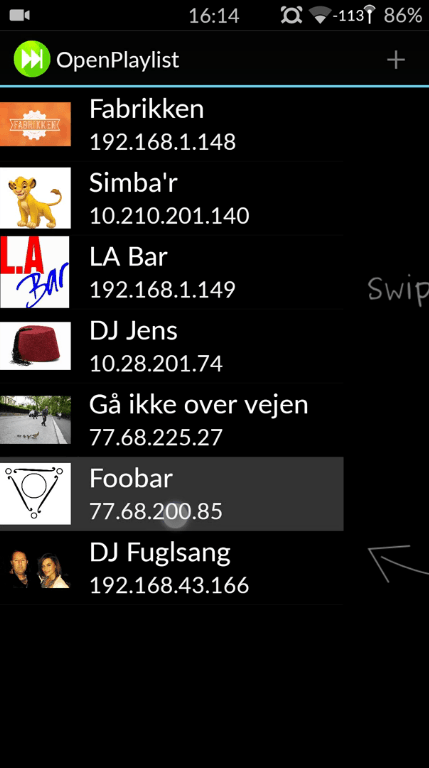
\includegraphics[width=0.3\linewidth]{ip}
  \caption{IP-address shown under each venue.}\label{fig:ip}
\end{figure}

\noindent\textbf{Problem \#11 - Confusion about which votes were made by users and which were
    votes made by the bar. Test person \#2.}\\
  During the usability tests, an environment simulator would vote on
  songs. This affected the playlist being displayed on the test
  device. It was however unclear to the test subject that these votes
  were also user votes and not bar votes.\\

\noindent\textbf{Problem \#12 - Did not know what tracks in a search already existed on the
    playlist. Test person \#2.}\\
  When searching for tracks, no visual confirmation was given whether
  the searched track was already on the playlist.\\

\noindent\textbf{Problem \#13 - Was confused why the search did not
  clear when the user made a new search. Test person \#2.}\\
  When a new search was performed right after a previous search, the
  search results of the new search would only display when the search
  was complete. The test subject expected the previous search results
  to disappear when the new search was conducted.\\

\noindent\textbf{Problem \#14 - Excepted ability to get more info when interacting with all
    tracks. Test person \#5.}\\
  One test subject was several times trying to interact with the
  tracks on the playlist in order to get additional information. This
  feature was not implemented.

\subsection{Usability Test Summary}
As no critical problems were found in the use of the system and all participants were able to complete all the tasks. The usability of the system is concluded to be good, but certainly not perfect. The problems found can be discussed and eventually solved, leading to a more usable system.

It was decided to fix problem \#1, \#2, \#3, \#4, \#5, \#6 and
\#10. These problems were chosen to cover all serious problems and
some of the most common minor problems. The final version of the
client application had these problems fixed. After the fixes, a new test
could be conducted in order to confirm that the problems was indeed
fixed, but this was dropped due to time constraints. The resisting problems are cosmetic, which mean that they do not influence the functionality of the application. It has been decided to delimit from these problems, due to limited time. 

While fixing problems \#4 and \#5, confirmation was added when adding
tracks from the search view and when checking into a venue. This results in a slightly different
interaction with the application, as the application will now forward
the user to a different screen upon adding tracks and checking into a venue.

\section{Unit Testing}
\label{unitTesting}
In this section, a description of the unit tests, which were constructed in an effort to check the quality and correctness of the software solution described in this report, will be presented.

\subsection{What is Unit Testing?}
Unit testing is a way of dividing code into small portions, which can then independently be tested for correctness\cite{unittesting}.

Unit tests should be quick, meaning that a developer can verify whether or not the code is correct, during development, without having to disrupt his work flow, to wait for the results.
Unit tests should also be small, checking only a single or very small subset of the functionality of the systems code.
Lastly, and perhaps most importantly, unit tests should be correct. If a unit test gives a false positive\footnote{A \emph{false positive} is when a test indicates that a condition is true, when, in reality, the condition is false. Likewise, a \emph{false negative} is when a test indicates a condition being false, when it is true.} then a developer would likely be convinced that the code which has been produced is working as it should, when in reality it is not. This could potentially lead to a logical error breaking the application on the end users' devices, among other undesirable situations. Likewise, if a unit test gives a false negative, a developer could waste a lot of time refactoring code, rewriting algorithms and modifying logic, even though the code was correct.


\subsection{Unit Testing for openPlaylist}
Unit testing in the system described in this report was implemented mostly on the server side. This was done, as the server side of openPlaylist is much more extensive than the rather dumb client.
The unit tests which were implemented covered various parts of the code, some test the correctness of methods, others verify connections to third party servers and some verify type extensions.
Unit tests for this project were implemented using xUnit.net\footnote{\url{http://xunit.github.io/}}, a powerful tool set for building unit tests in the .Net framework. In xUnit.net, most unit tests are created using assertions, which check that a certain condition is met and if not, fails the test.
To run the unit tests, a developer simply has to click the \enquote{Run All}-button in the Test Explorer in Visual Studio. This gives the developer a quick overview of the unit tests and whether or not they have passed, as can be seen in \cref{fig:UnitTestsPassed}.

\begin{figure}[H]
  \centering
  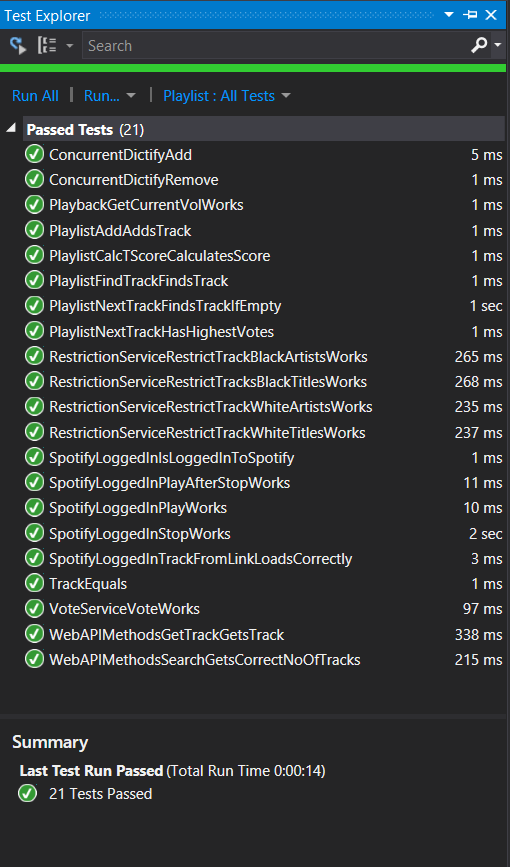
\includegraphics[width=.7\textwidth]{UnitTestsPassed.png}
  \caption{The Test Explorer in Visual Studio.}\label{fig:UnitTestsPassed}
\end{figure}

As can be seen in \cref{lst:UnitTest}, the unit tests which were implemented in the software solution were fairly simple. The example shows the manual creation of a \emph{Track} and a call to a method, which will automatically get the \emph{Track}. The test is simply an assertion that the two \emph{Track}s are identical. In \cref{fig:UnitTestsPassed}, it can be seen that this assertion is indeed true and the test has passed. This should mean that the method for automatically getting a \emph{Track} works as it should.
It should be noted that the method for getting a \emph{Track} uses a third party database. This means that, in a situation where the database has modified the data for this particular \emph{Track}, the test would fail, as it would not be equal to the manually constructed \emph{Track}. However, if the test passes, it is extremely unlikely that the method, which is tested, is incorrect.

\begin{lstlisting}[float, floatplacement=htpb,caption = {Test method for the automatic getting of a \textbf{Track}}, label = {lst:UnitTest}]
[Fact]
public void WebAPIMethodsGetTrackGetsTrack()
{
	(...)
	var track = new Track("19pTAbMZmWsgGkYZ4v2TM1", "Obliteration of the Weak", 232120, false, 1, "DKFD51642001" , "https://p.scdn.co/mp3-preview/1d3ee1111d679b5e5b50c53aa3bfcceb4c83da8a", alb);

	var foundTrack = WebAPIMethods.GetTrack(track.URI);

	Assert.Equal(track, foundTrack);
}
\end{lstlisting}



\section{Implementing the User Interface}\label{sec:impinterface}
As stated in \cref{sec:serverInterface} the usability of the server interface was not considered. Therefore this section focus on explaining how previously explained functionality is implemented and can be achieved by the administrator.

The first screen the administrator meets when opening the application is the login screen for spotify, as seen in \cref{fig:loginInterface}. Here the administrator inputs the login credentials for the venues Business Spotify Account (see \cref{ch:preface} for legal terms). This is used to get the data needed to play songs from spotify's catalogue. From this interface the administrators and stop and start the playback of music as described in \cref{systemDefinition}. Also the icon for the application acts as a skip button where administrators can skip the currently playing track.

\begin{figure}[H]\label{fig:loginInterface}
  \centering
  \subfloat{
    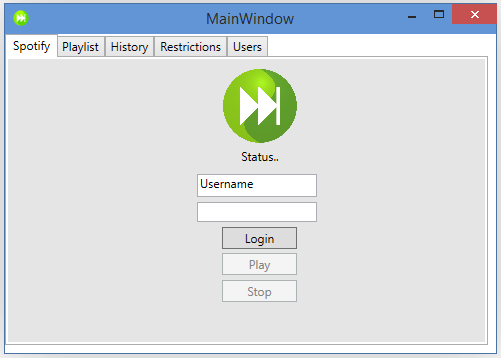
\includegraphics[width=0.5\textwidth]{ServerInterfaceLogin}
  }
  \subfloat{
    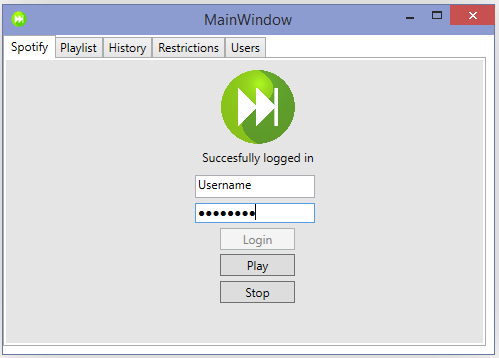
\includegraphics[width=0.5\textwidth]{ServerInterfaceLoggedin}
  }
  \caption{Login interface on the server.}
\end{figure}

The second interface is the playlist and can be seen in \cref{fig:ServerInterfacePlaylist}. Here the most crucial information about tracks on the playlist can be seen; the title, artist(s), duration (in milliseconds), temporary and permanent votes. The album cover is also displayed for the ability to quickly identify tracks. The playlist is ordered in the order they will be played, the higher a placement, the sooner it will be played. From this interface further administrative control can be executed including removal of specific tracks and rearrangement of the playlist as described in \cref{systemDefinition}. When pressing the move up or move down button the currently selected track changes one position, this is done through changing the permanent votes just enough for the track to change place.

\begin{figure}[hbtp]
  \centering
  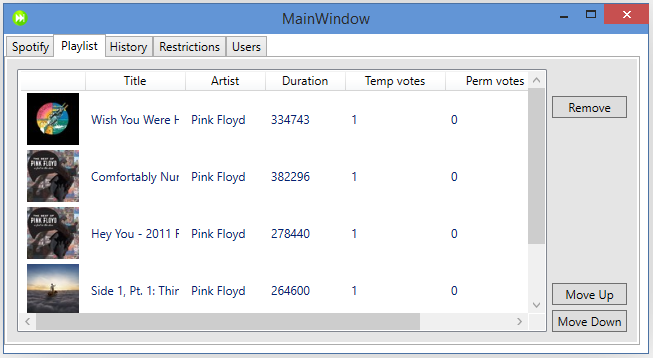
\includegraphics[width=\textwidth]{Images/ServerInterfacePlaylist.png}
  \caption{Playlist interface on the server.}\label{fig:ServerInterfacePlaylist}
\end{figure}

The third interface is the history interface, seen in \cref{fig:ServerInterfaceHistory}. From here the administrator can see what was been played previously. The higher on the list the longer ago it has been played. Like the playlist interface only the most crucial information is displayed, therefore all votes are removed since these are not important any longer.

\begin{figure}[hbtp]
  \centering
  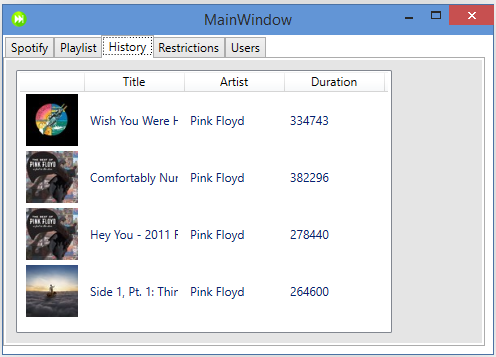
\includegraphics[width=\textwidth]{Images/ServerInterfaceHistory.png}
  \caption{History interface on the server.}\label{fig:ServerInterfaceHistory}
\end{figure}

The fourth interface is the restriction interface and can be seen in \cref{fig:ServerInterfaceRestrictions1}. from here the administrator can modify, remove and add restrictions. Adding or modifying a restriction brings up a dialogue where parameters for the restriction according to \cref{sec:restrictions}.

\begin{figure}[H]
  \centering
  \subfloat[Main restriction interface.]{
    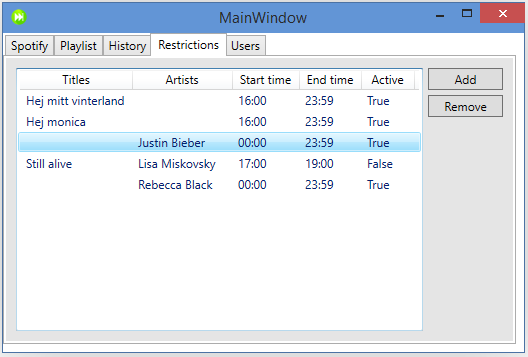
\includegraphics[height=160px]{ServerInterfaceRestrictions}
        \label{fig:ServerInterfaceRestrictions1}
  }
  \subfloat[Restriction modify dialogue.]{
    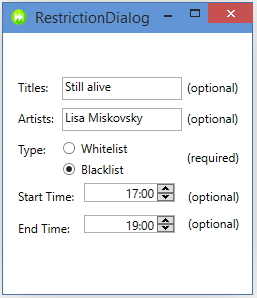
\includegraphics[height=160px]{ServerInterfaceRestrictionDialog}
        \label{fig:ServerInterfaceRestrictions2}
  }
  \caption{Restriction interface on the server.}
\end{figure}

The last interface is the user interface and can be seen in \cref{fig:ServerInterfaceUsers}. From here the administrator can keep track of how many and which guests have checked in at the venue. The administrator can see what they have voted, both an track and volume. The guests should here be represented via their unique ID as will be described in \cref{sec:UAuth}
\begin{figure}[hbtp]
  \centering
  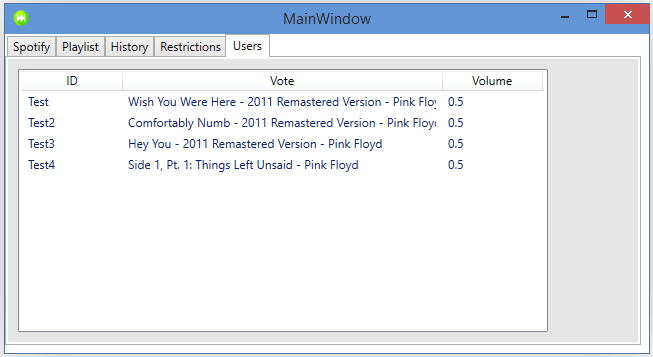
\includegraphics[width=\textwidth]{Images/ServerInterfaceUsers.png}
  \caption{User interface on the server.}\label{fig:ServerInterfaceUsers}
\end{figure}

